\documentclass[a4paper,12pt]{article}
\usepackage{amsmath}
\usepackage{enumerate}
\usepackage{graphicx}

\pagestyle{empty} \setlength{\parindent}{0mm}
\addtolength{\topmargin}{-0.5in} \setlength{\textheight}{9in}
\addtolength{\textwidth}{1in} \addtolength{\oddsidemargin}{-0.5in}


\begin{document}
\title{Final Homework}
\author{Matt Forbes}
\date{December 7, 2010}
\maketitle

\section*{Problem 1}

\begin{enumerate}[]
  
\item The cost of going from exit $j$ to $k$ is $C_j + C_{j+1} +
  C_{j+2} + \dots + C_{k-1}$. I propose the data structure $H$ such
  that $H_i = C_1 + C_2 + \dots + C_{i-1}$. To calculate the cost exit
  $j$ to $k$ using $H$, it would simply be $H_k - H_j$. This
  expression expands to $(C_1 + C_2 + \dots + C_{j-1}) - (C_1 + C_2 +
  \dots + C_{k-1})$, which simplifies to $C_j + C_{j+1} + \dots +
  C_{k-1}$. Showing that $H_k - H_j$ is equivalent to the cost we
  calculated for exit $j$ to $k$. Given that $H$ is already
  calculated, this computation is a simple subtraction, $O(1)$.

\item Generating this data structure is very easy and would take
  $O(n)$ time and holds $n$ elements. Each element $H_i$ is equal to
  $C_i + H_{i-1}$ which lends itself easily to an accumlating loop
  from $1$ to $n$.

\item
\begin{verbatim}
H[1] = C[1]
for i = 2...n:
  H[i] = C[i] + H[i-1]
\end{verbatim}
  
\end{enumerate}

\section*{Problem 2}

\begin{center}
  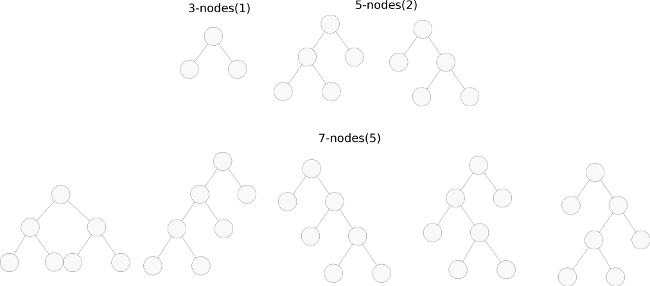
\includegraphics[width=450px, height=225px, keepaspectratio=true]{image/fulltrees.png}
\end{center}

\begin{enumerate}[a)]

\item $B_3 = 1, B_5 = 2, B_7 = 5$.

\item You can't construct a full binary tree with an even number of
  nodes. Every node always has zero or two child nodes, meaning
  everytime the tree grows, it must grow by a multiple of two
  nodes. So starting with the root, and growing $n$ times, the total
  number of nodes will always be of the form $1 + 2n$, which is odd.

\item

  \begin{enumerate}[]
    
  \item Before determining an upper bound for the number of full
    binary trees of some size, it is necessary to know how many leaves
    such a tree has. All full binary trees of size $n$ can be built by
    simply adding two nodes as the left and right child to any leaf
    node on a tree of size $n-2$. For this reason, all full trees with
    the same number of nodes have the same number of leaves.

  \item Starting from the most simple full tree of size 3, it can be
    seen that every time the tree grows (by two nodes), the number of
    leaves increases by one. This is because to grow the tree, two
    nodes must fill a leaf's children, which results in one more leaf
    than before. So the number of leaves on a full tree of size $k$ is
    just the number of times two leaves were added to the tree of
    three nodes plus the original two on that tree. So as a function
    of $k$, the number of leaves of a full tree, $L_k$, is $L_k = 2 +
    \frac{k-3}{2}$. The first term is the original two leaves on the
    base tree, and $\frac{k-3}{2}$ is the number of times two nodes
    were added to the base tree.

  \item With this expression for the number of leaves in a full tree,
    we can now discuss the number of full trees of size $n$. All of
    these trees of size $n$ had to be constructed by growing some
    smaller tree with $n-2$ nodes. Assuming that we know $B_{n-2}$,
    then $B_n \le L_{n-2}B_{n-2}$. This is just the number of trees
    multiplied by the number of leaves on each tree, which constructs
    every possible tree of size $n$.

  \item Expanding this expression we get:
    \begin{align*}
      B_n &= L_{n-2}B_{n-2}\\
      &= (2 + \frac{(n-2) - 3}{2})B_{n-2}\\
      &= 2B_{n-2} + (\frac{n-5}{2})B_{n-2}
    \end{align*}
    

  \item 
    

  \end{enumerate}

\end{enumerate}


\section*{Problem 3}


\begin{verbatim}
  structure weirdqueue {
     pushstack (stack pointer)
     popstack (stack pointer)
  }

  def enqueue(Q, elt):
     Q.pushstack.push(elt)

  def dequeue(Q):
     if Q.pushstack and Q.popstack are empty:
        error underflow
     if Q.popstack is empty:
        while Q.pushstack is not empty:
           Q.popstack.push( Q.pushstack.pop() )
        swap Q.popstack pointer with Q.pushstack
     return Q.popstack.pop()

\end{verbatim}


\begin{enumerate}[a)]

\item Under the assumption that the 'popstack' is empty, we would have
  to pop each element off the 'pushstack' and then push that on to the
  'popstack.' By doing this we are reversing the order, guaranteeing
  that we get the first queued item, but means we are also doing work
  proportional to the size of the structure, $O(n)$.

\item In practice, we could not possibly have to do this mass popping
  and pushing to reorient the structure every dequeue. This means that
  we will have a much faster amortized analysis of the running
  time. If we follow the lifetime of one element in the structure,
  there are only about 4 operations associated with it. We initially
  push it on to the 'pushstack' and then at some later time we will
  transfer it to the 'popstack' and finally pop it one more time when
  it is removed. So there can never be more than 4 operations per
  element lifecycle. Using amortized analysis, we can see that $n$
  insertions could never be worse than about $4n$ stack
  operations. Therefore, the average cost per enqueue/dequeue
  operation is $\frac{4n}{n} = 4$, which is $O(1)$.
  
\end{enumerate}

\section*{Problem 4}

\begin{enumerate}[a)]

\item
  \begin{enumerate}[]
    
  \item I'm not quite sure how to go about analyzing this
    algorithm. There really seems to be a lot of dependencies, and I'm
    not yet skilled in the art of probability. My best attempt was to
    try partition the bets in to two groups: the first $\frac{n}{10}$
    and the rest. If we call the largest bid in the first partition
    $M$, and let the list of bets, $L$, be all the bets in the second
    partition that are greater than $M$, we can find the
    probability. Assuming that we can find this list $L$, or even the
    number of elements in it then the probability of picking the
    highest bet is equal to the probability that the highest bet is
    the first element of $L$.

  \item So, the probabiliy of taking the highest bet is
    $\dfrac{1}{\text{length}(L)}$, where $L$ is the list described
    above (number of bets in the partition that are greater than
    maximum of first).

  \item Now we have some way of determining the probability, albeit
    one that assumes a lot. I really don't know how to go about
    determining the length of $L$ formally, but we can analyze the
    smallest and largest values it can take. First of all, the worst
    case is that the $\frac{n}{10}$ smallest elements are the first
    bets in the sequence. In that case {\italics all} the bets in the
    second partition are greater than the maximum of the
    first. Therefore, the probability of picking the highest bid would
    be $\dfrac{1}{\frac{9n}{10}} = \dfrac{10}{9n}$ in this scenario.

  \item On the other hand, if the $2^{nd}$ largest bet was one of the
    first $\frac{n}{10}$ bets seen, then we are guaranteed to accept
    the very highest bet. So in this case, the probability is $1$.

  \end{enumerate}

\end{enumerate}


\end{document}
